\chapter{Method}
\label{ch:method}

\section{The dataset}
The dataset consists of manually labeled recorded movies of 20 different people
performing the complete sequence of hand poses.

Usually the 12 Curwen solfege hand symbols are performed in front of the torso
as shown in Figure~\ref{fig:hands_normal}. To increase the number of hand poses
to be recogniced, all 12 Curwen are also performed mirrored next to the body of
the recorded subject, see Figure~\ref{fig:hands_mirrored}. Additionally four
extra hand symbols have been added that are not part of the Curwen sequence, see
Figure~\ref{fig:hands_extra}. These last four symbols are performed next to the
head.


\renewcommand{\thesubfigure}{\thefigure.\roman{subfigure}} 
\begin{figure}[htbp]
\begin{center}
\subfloat[Do]{\label{fig:hand_0}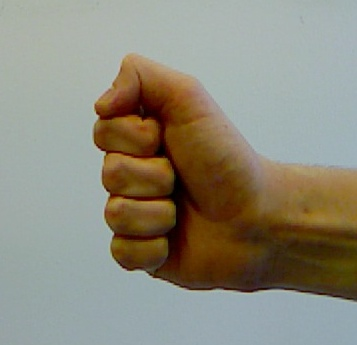
\includegraphics[width=0.2\linewidth,height=0.15\linewidth]{figures/examples/0.jpg}}
\hspace{0.03\linewidth}
\subfloat[Di]{\label{fig:hand_1}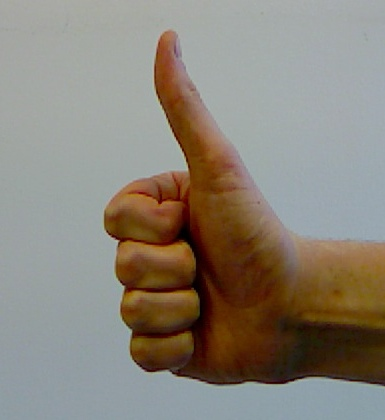
\includegraphics[width=0.2\linewidth,height=0.15\linewidth]{figures/examples/1.jpg}}
\hspace{0.03\linewidth}
\subfloat[Re]{\label{fig:hand_2}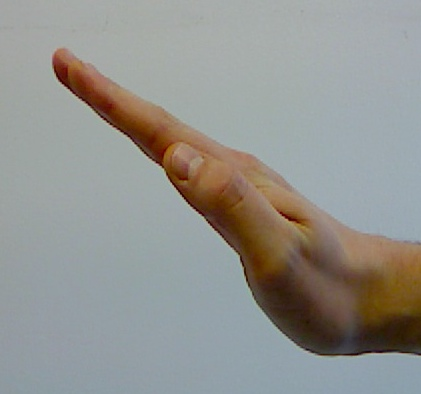
\includegraphics[width=0.2\linewidth,height=0.15\linewidth]{figures/examples/2.jpg}}
\hspace{0.03\linewidth}
\subfloat[Ri]{\label{fig:hand_3}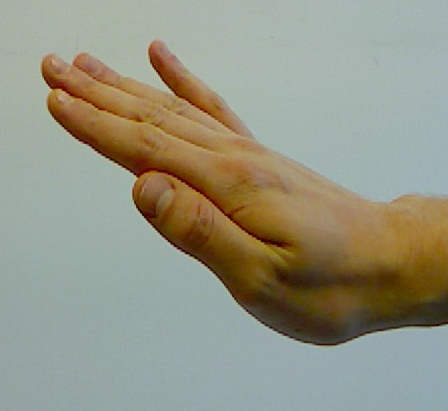
\includegraphics[width=0.2\linewidth,height=0.15\linewidth]{figures/examples/3.jpg}}
\hspace{0.03\linewidth}
\subfloat[Mi]{\label{fig:hand_4}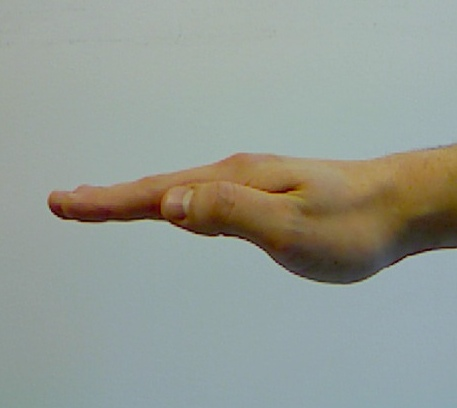
\includegraphics[width=0.2\linewidth,height=0.15\linewidth]{figures/examples/4.jpg}}
\hspace{0.03\linewidth}
\subfloat[Fa]{\label{fig:hand_5}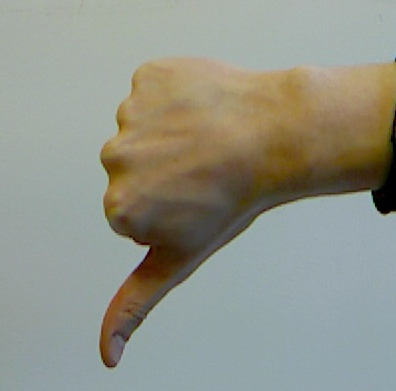
\includegraphics[width=0.2\linewidth,height=0.15\linewidth]{figures/examples/5.jpg}}
\hspace{0.03\linewidth}
\subfloat[Fi]{\label{fig:hand_6}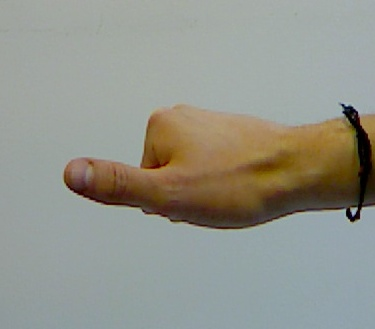
\includegraphics[width=0.2\linewidth,height=0.15\linewidth]{figures/examples/6.jpg}}
\hspace{0.03\linewidth}
\subfloat[Sol]{\label{fig:hand_7}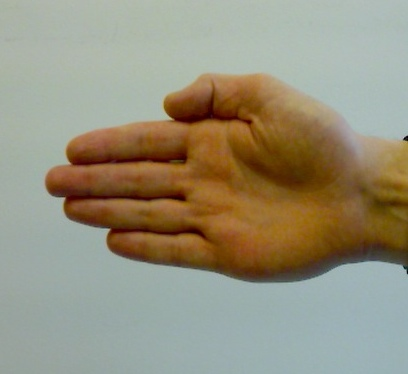
\includegraphics[width=0.2\linewidth,height=0.15\linewidth]{figures/examples/7.jpg}}
\hspace{0.03\linewidth}
\subfloat[Si]{\label{fig:hand_8}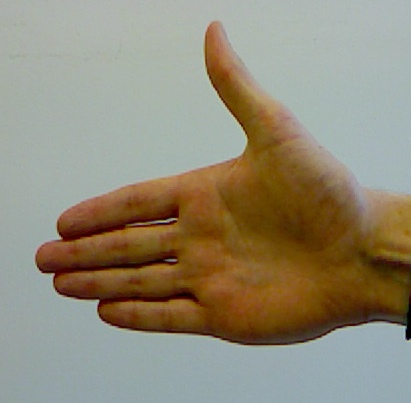
\includegraphics[width=0.2\linewidth,height=0.15\linewidth]{figures/examples/8.jpg}}
\hspace{0.03\linewidth}
\subfloat[La]{\label{fig:hand_9}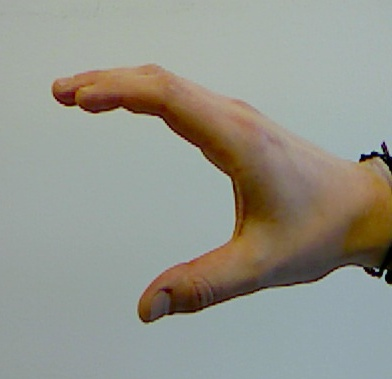
\includegraphics[width=0.2\linewidth,height=0.15\linewidth]{figures/examples/9.jpg}}
\hspace{0.03\linewidth}
\subfloat[Li]{\label{fig:hand_10}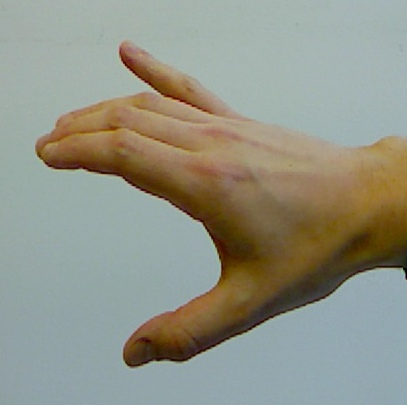
\includegraphics[width=0.2\linewidth,height=0.15\linewidth]{figures/examples/10.jpg}}
\hspace{0.03\linewidth}
\subfloat[Ti]{\label{fig:hand_11}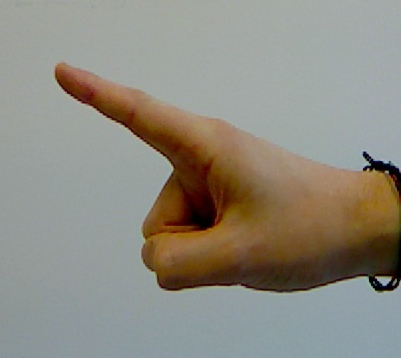
\includegraphics[width=0.2\linewidth,height=0.15\linewidth]{figures/examples/11.jpg}}
\end{center}
\caption{All mirrored Curwen hand poses}
\label{fig:hands_mirrored}
\end{figure}

\begin{figure}[htbp]
\begin{center}
\subfloat[Do]{\label{fig:hand_12}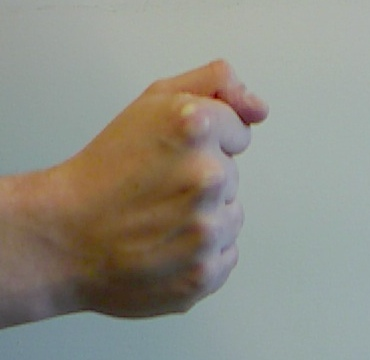
\includegraphics[width=0.2\linewidth,height=0.15\linewidth]{figures/examples/12.jpg}}
\hspace{0.03\linewidth}
\subfloat[Di]{\label{fig:hand_13}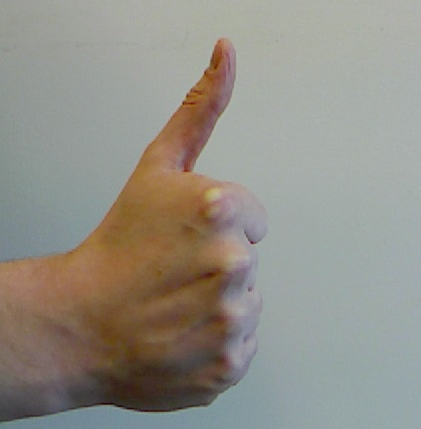
\includegraphics[width=0.2\linewidth,height=0.15\linewidth]{figures/examples/13.jpg}}
\hspace{0.03\linewidth}
\subfloat[Re]{\label{fig:hand_14}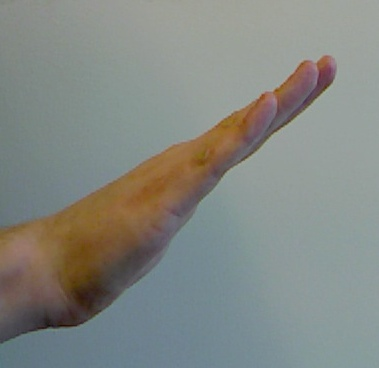
\includegraphics[width=0.2\linewidth,height=0.15\linewidth]{figures/examples/14.jpg}}
\hspace{0.03\linewidth}
\subfloat[Ri]{\label{fig:hand_15}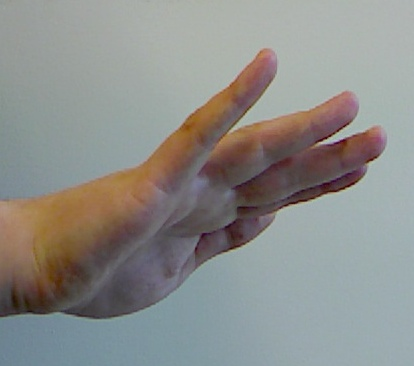
\includegraphics[width=0.2\linewidth,height=0.15\linewidth]{figures/examples/15.jpg}}
\hspace{0.03\linewidth}
\subfloat[Mi]{\label{fig:hand_16}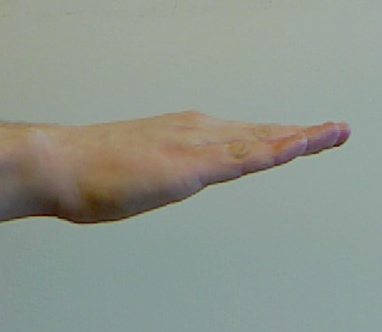
\includegraphics[width=0.2\linewidth,height=0.15\linewidth]{figures/examples/16.jpg}}
\hspace{0.03\linewidth}
\subfloat[Fa]{\label{fig:hand_17}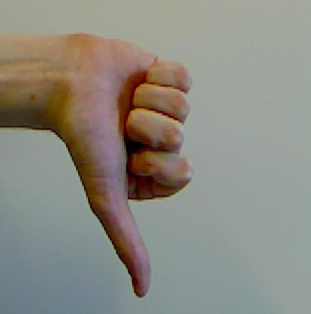
\includegraphics[width=0.2\linewidth,height=0.15\linewidth]{figures/examples/17.jpg}}
\hspace{0.03\linewidth}
\subfloat[Fi]{\label{fig:hand_18}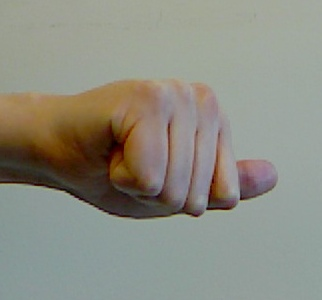
\includegraphics[width=0.2\linewidth,height=0.15\linewidth]{figures/examples/18.jpg}}
\hspace{0.03\linewidth}
\subfloat[Sol]{\label{fig:hand_19}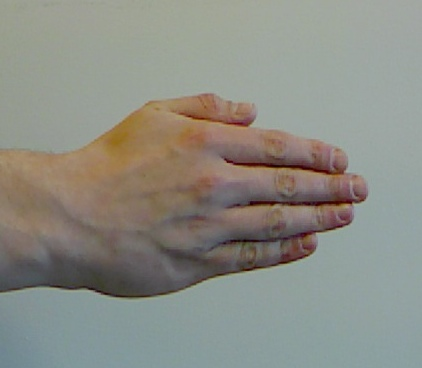
\includegraphics[width=0.2\linewidth,height=0.15\linewidth]{figures/examples/19.jpg}}
\hspace{0.03\linewidth}
\subfloat[Si]{\label{fig:hand_20}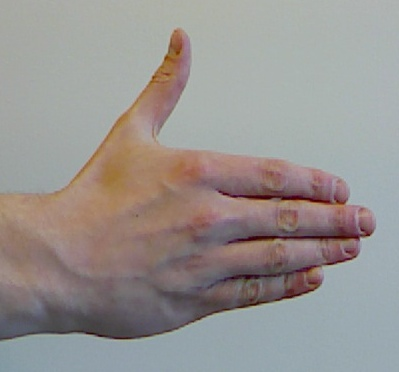
\includegraphics[width=0.2\linewidth,height=0.15\linewidth]{figures/examples/20.jpg}}
\hspace{0.03\linewidth}
\subfloat[La]{\label{fig:hand_21}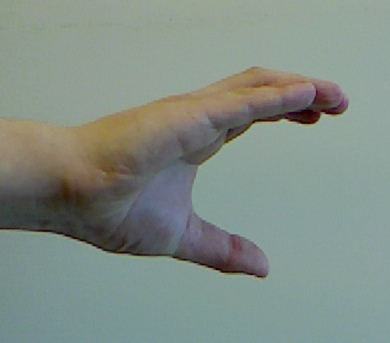
\includegraphics[width=0.2\linewidth,height=0.15\linewidth]{figures/examples/21.jpg}}
\hspace{0.03\linewidth}
\subfloat[Li]{\label{fig:hand_22}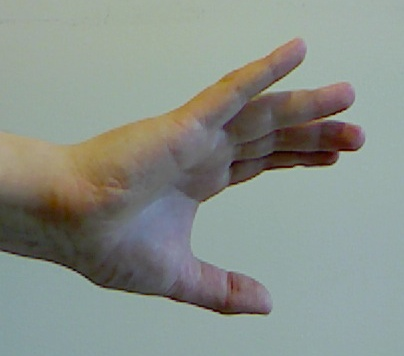
\includegraphics[width=0.2\linewidth,height=0.15\linewidth]{figures/examples/22.jpg}}
\hspace{0.03\linewidth}
\subfloat[Ti]{\label{fig:hand_23}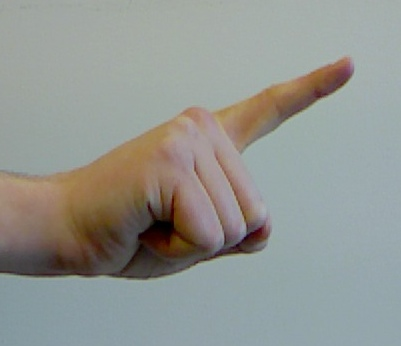
\includegraphics[width=0.2\linewidth,height=0.15\linewidth]{figures/examples/23.jpg}}
\end{center}
\caption{All Curwen hand poses}
\label{fig:hands_normal}
\end{figure}


\begin{figure}[htbp]
\begin{center}
\subfloat[Extra1]{\label{fig:hand_24}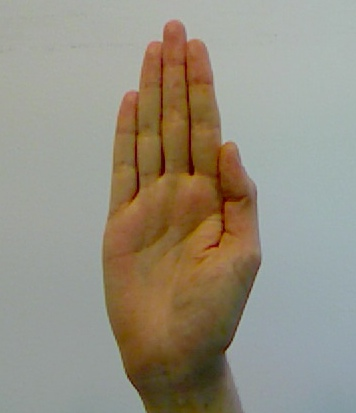
\includegraphics[width=0.2\linewidth,height=0.15\linewidth]{figures/examples/24.jpg}}
\hspace{0.03\linewidth}
\subfloat[Extra2]{\label{fig:hand_25}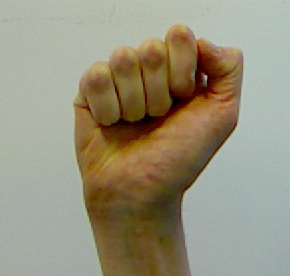
\includegraphics[width=0.2\linewidth,height=0.15\linewidth]{figures/examples/25.jpg}}
\hspace{0.03\linewidth}
\subfloat[Extra3]{\label{fig:hand_26}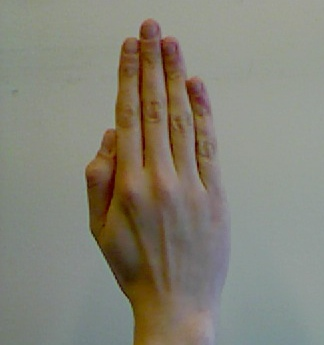
\includegraphics[width=0.2\linewidth,height=0.15\linewidth]{figures/examples/26.jpg}}
\hspace{0.03\linewidth}
\subfloat[Extra4]{\label{fig:hand_27}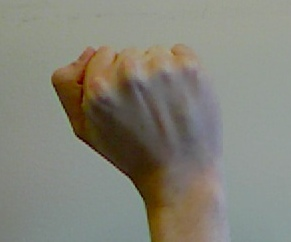
\includegraphics[width=0.2\linewidth,height=0.15\linewidth]{figures/examples/27.jpg}}
\end{center}
\caption{The extra hand poses}
\label{fig:hands_extra}
\end{figure}


\begin{figure}[htbp]
\begin{center}
\subfloat[Do]{\label{fig:gijs5_0}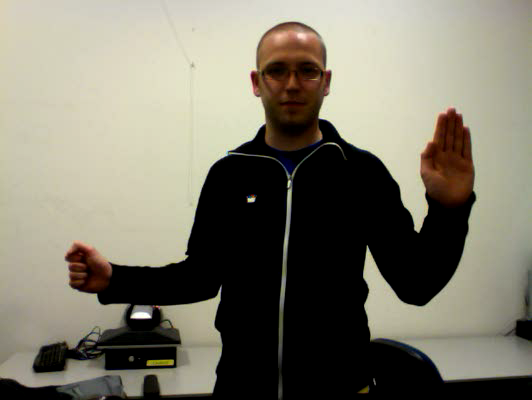
\includegraphics[width=0.2\linewidth,height=0.15\linewidth]{figures/gijs5/0.png}}
\hspace{0.03\linewidth}
\subfloat[Di]{\label{fig:gijs5_1}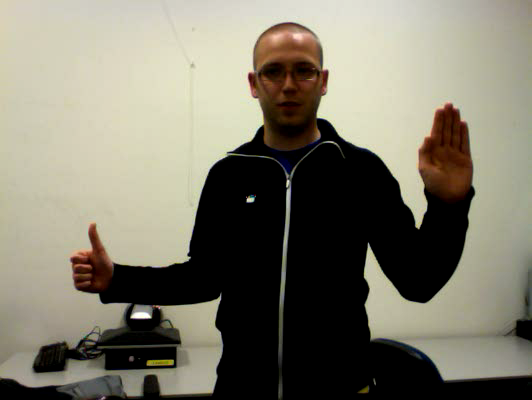
\includegraphics[width=0.2\linewidth,height=0.15\linewidth]{figures/gijs5/1.png}}
\hspace{0.03\linewidth}
\subfloat[Re]{\label{fig:gijs5_2}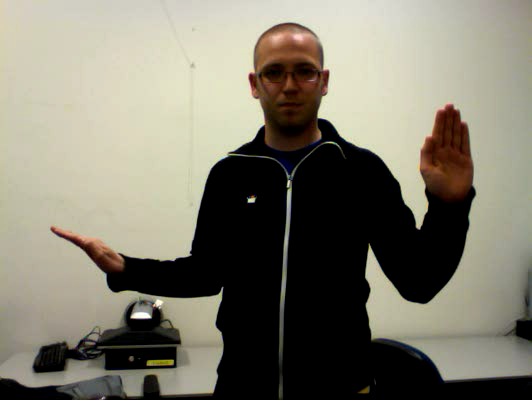
\includegraphics[width=0.2\linewidth,height=0.15\linewidth]{figures/gijs5/2.png}}
\hspace{0.03\linewidth}
\subfloat[Ri]{\label{fig:gijs5_3}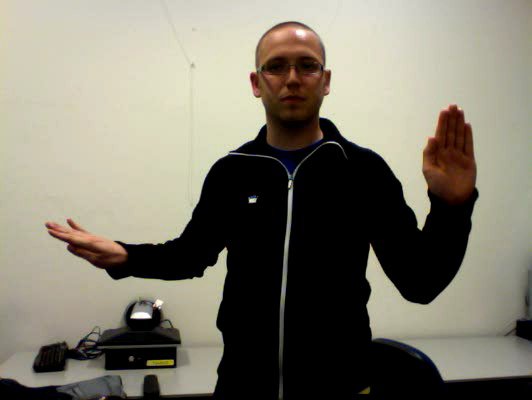
\includegraphics[width=0.2\linewidth,height=0.15\linewidth]{figures/gijs5/3.png}}
\hspace{0.03\linewidth}
\subfloat[Mi]{\label{fig:gijs5_4}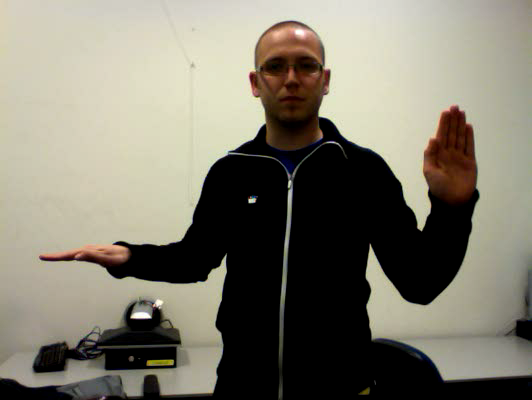
\includegraphics[width=0.2\linewidth,height=0.15\linewidth]{figures/gijs5/4.png}}
\hspace{0.03\linewidth}
\subfloat[Fa]{\label{fig:gijs5_5}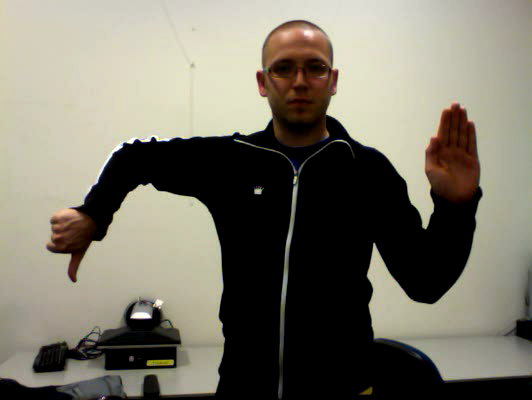
\includegraphics[width=0.2\linewidth,height=0.15\linewidth]{figures/gijs5/5.png}}
\hspace{0.03\linewidth}
\subfloat[Fi]{\label{fig:gijs5_6}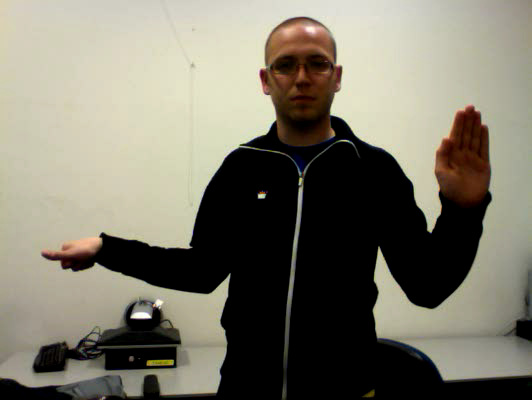
\includegraphics[width=0.2\linewidth,height=0.15\linewidth]{figures/gijs5/6.png}}
\hspace{0.03\linewidth}
\subfloat[Sol]{\label{fig:gijs5_7}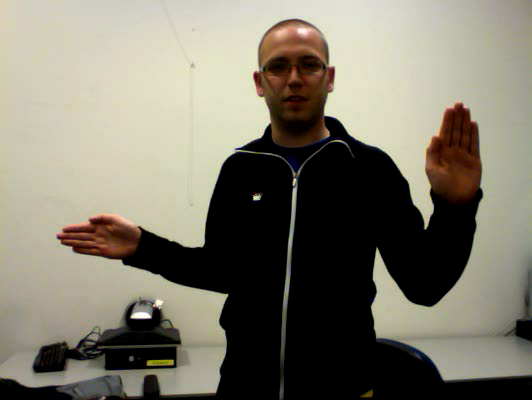
\includegraphics[width=0.2\linewidth,height=0.15\linewidth]{figures/gijs5/7.png}}
\hspace{0.03\linewidth}
\subfloat[Si]{\label{fig:gijs5_8}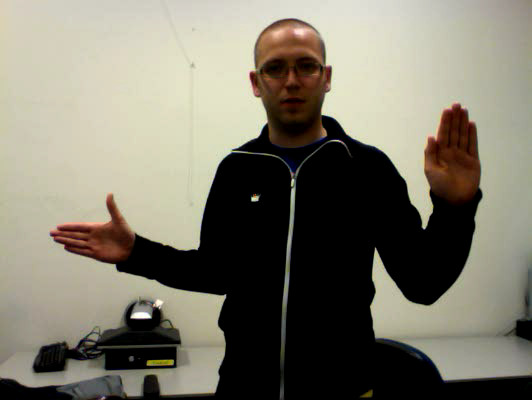
\includegraphics[width=0.2\linewidth,height=0.15\linewidth]{figures/gijs5/8.png}}
\hspace{0.03\linewidth}
\subfloat[La]{\label{fig:gijs5_9}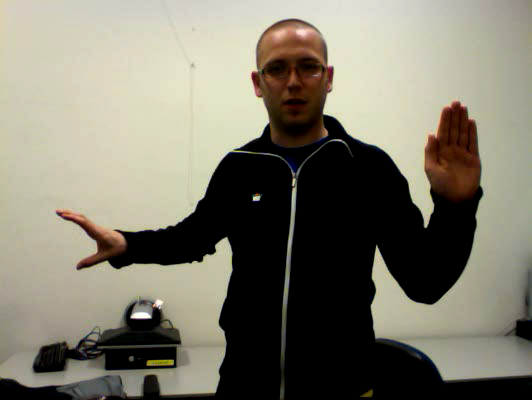
\includegraphics[width=0.2\linewidth,height=0.15\linewidth]{figures/gijs5/9.png}}
\hspace{0.03\linewidth}
\subfloat[Li]{\label{fig:gijs5_10}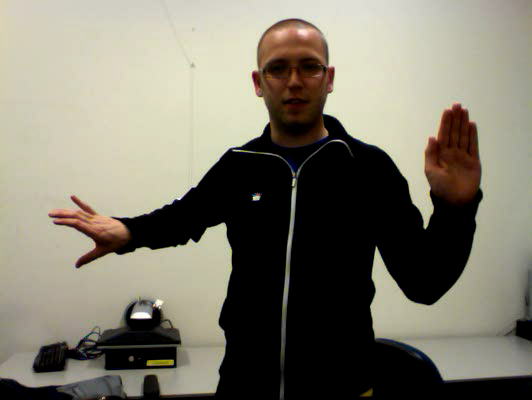
\includegraphics[width=0.2\linewidth,height=0.15\linewidth]{figures/gijs5/10.png}}
\hspace{0.03\linewidth}
\subfloat[Ti]{\label{fig:gijs5_11}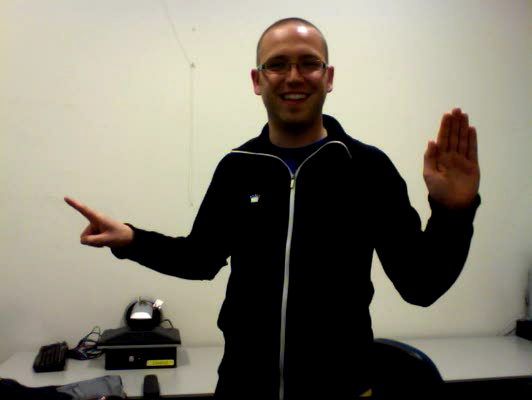
\includegraphics[width=0.2\linewidth,height=0.15\linewidth]{figures/gijs5/11.png}}
\hspace{0.03\linewidth}
\subfloat[Do]{\label{fig:gijs5_12}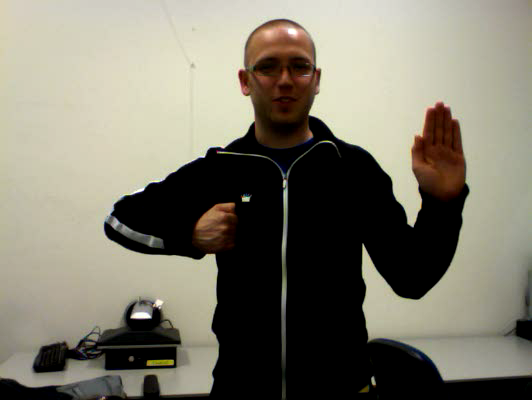
\includegraphics[width=0.2\linewidth,height=0.15\linewidth]{figures/gijs5/12.png}}
\hspace{0.03\linewidth}
\subfloat[Di]{\label{fig:gijs5_13}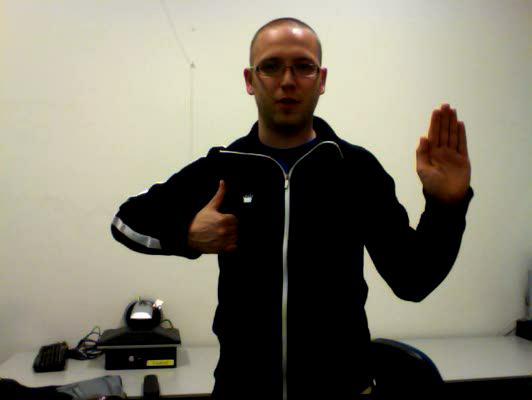
\includegraphics[width=0.2\linewidth,height=0.15\linewidth]{figures/gijs5/13.png}}
\hspace{0.03\linewidth}
\subfloat[Re]{\label{fig:gijs5_14}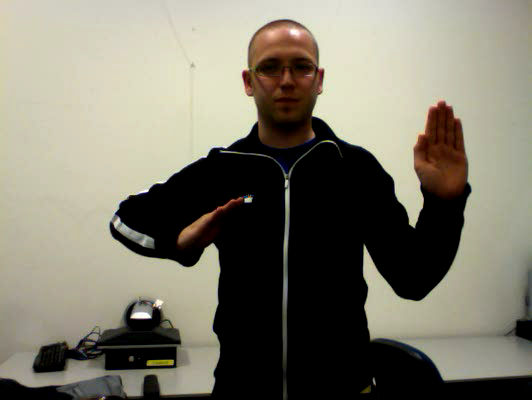
\includegraphics[width=0.2\linewidth,height=0.15\linewidth]{figures/gijs5/14.png}}
\hspace{0.03\linewidth}
\subfloat[Ri]{\label{fig:gijs5_15}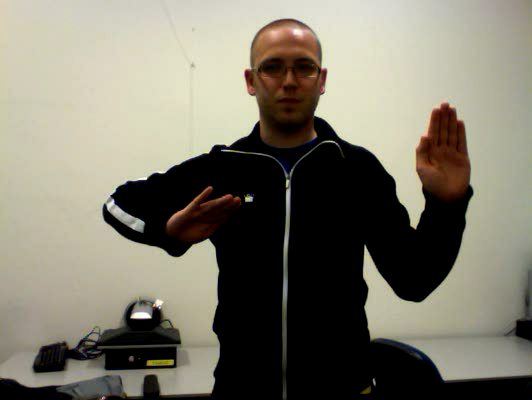
\includegraphics[width=0.2\linewidth,height=0.15\linewidth]{figures/gijs5/15.png}}
\hspace{0.03\linewidth}
\subfloat[Mi]{\label{fig:gijs5_16}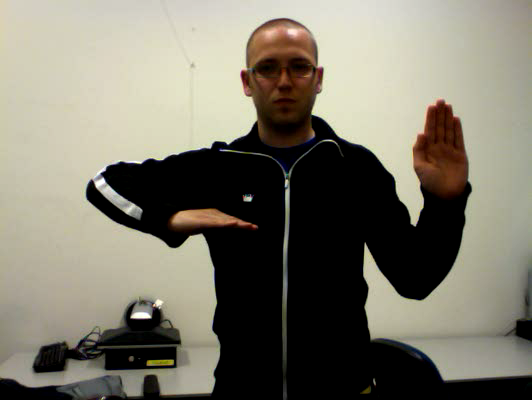
\includegraphics[width=0.2\linewidth,height=0.15\linewidth]{figures/gijs5/16.png}}
\hspace{0.03\linewidth}
\subfloat[Fa]{\label{fig:gijs5_17}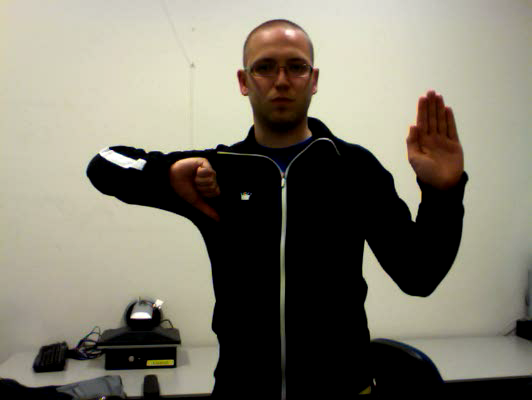
\includegraphics[width=0.2\linewidth,height=0.15\linewidth]{figures/gijs5/17.png}}
\hspace{0.03\linewidth}
\subfloat[Fi]{\label{fig:gijs5_18}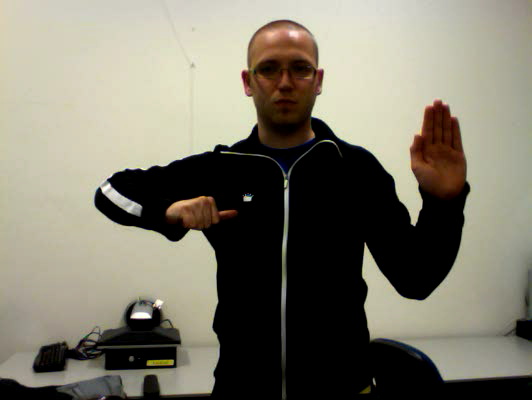
\includegraphics[width=0.2\linewidth,height=0.15\linewidth]{figures/gijs5/18.png}}
\hspace{0.03\linewidth}
\subfloat[Sol]{\label{fig:gijs5_19}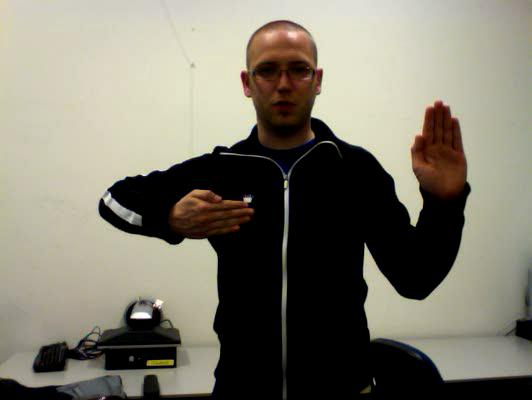
\includegraphics[width=0.2\linewidth,height=0.15\linewidth]{figures/gijs5/19.png}}
\hspace{0.03\linewidth}
\subfloat[Si]{\label{fig:gijs5_20}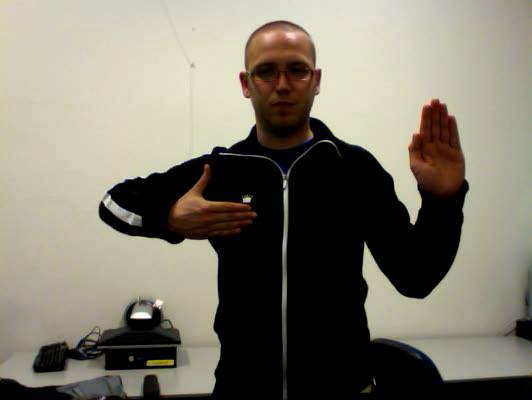
\includegraphics[width=0.2\linewidth,height=0.15\linewidth]{figures/gijs5/20.png}}
\hspace{0.03\linewidth}
\subfloat[La]{\label{fig:gijs5_21}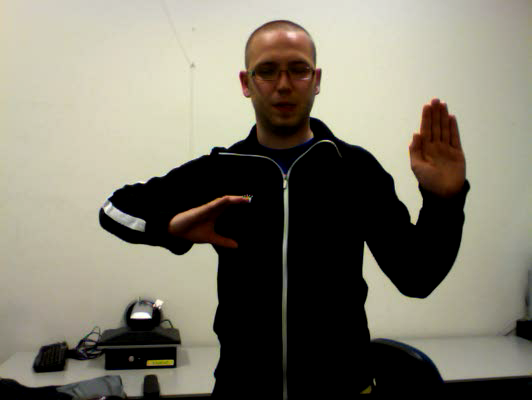
\includegraphics[width=0.2\linewidth,height=0.15\linewidth]{figures/gijs5/21.png}}
\hspace{0.03\linewidth}
\subfloat[Li]{\label{fig:gijs5_22}\includegraphics[width=0.2\linewidth,height=0.15\linewidth]{figures/gijs5/22.png}}
\hspace{0.03\linewidth}
\subfloat[Ti]{\label{fig:gijs5_23}\includegraphics[width=0.2\linewidth,height=0.15\linewidth]{figures/gijs5/23.png}}
\hspace{0.03\linewidth}
\subfloat[Extra1]{\label{fig:gijs5_24}\includegraphics[width=0.2\linewidth,height=0.15\linewidth]{figures/gijs5/24.png}}
\hspace{0.03\linewidth}
\subfloat[Extra2]{\label{fig:gijs5_25}\includegraphics[width=0.2\linewidth,height=0.15\linewidth]{figures/gijs5/25.png}}
\hspace{0.03\linewidth}
\subfloat[Extra3]{\label{fig:gijs5_26}\includegraphics[width=0.2\linewidth,height=0.15\linewidth]{figures/gijs5/26.png}}
\hspace{0.03\linewidth}
\subfloat[Extra4]{\label{fig:gijs5_27}\includegraphics[width=0.2\linewidth,height=0.15\linewidth]{figures/gijs5/27.png}}
\end{center}
\caption{Stills from recording number 5, test subject 'gijs'}
\label{fig:gijs5}
\end{figure}




\section{Evaluation}
